\chapter{Methodology}
\label{ch:methodology}

% ─────────────────────────────────────────────────────────────────────────────
\section{Research Design}
\label{sec:meth_design}
% ─────────────────────────────────────────────────────────────────────────────

This project adopts \textit{Design Science Research} (DSR) \parencite{hevner2004},
which prescribes iterative construction and evaluation of an artefact intended
to solve a practical problem. The artefact is GeoMentor: a production-deployed
adaptive ITS for UK KS3/GCSE Geography implementing a hybrid IRT 3PL + BKT
algorithm. The evaluation employs a within-subjects quasi-experimental design;
the absence of randomised group assignment (due to the convenience sample)
classifies the design as quasi-experimental rather than a true RCT.
The scope was concentrated on a single KC domain (UK physical geography and
climate, 13 KCs) following a Sprint~5 technical risk assessment, a decision
that strengthens rather than weakens evaluation claims: single-domain
validation depth produces more defensible psychometric evidence than shallow
multi-domain coverage.

% ─────────────────────────────────────────────────────────────────────────────
\section{Knowledge Representation}
\label{sec:meth_kc}
% ─────────────────────────────────────────────────────────────────────────────

\subsection{Knowledge Component Ontology}
\label{subsec:meth_kc_ontology}

The curriculum is decomposed into 13 Knowledge Components (KCs). A KC is a
unit of knowledge for which mastery can be operationally defined
\parencite{koedinger2012}. Table~\ref{tab:kc_table} lists all 13 KCs with
their Bloom ceiling and BKT prior parameters as implemented in
\texttt{DEFAULT\_BKT\_PARAMS}.

\begin{table}[H]
\centering
\caption{Knowledge Component ontology: 13 KCs with BKT prior parameters.
  $p(G) = 0.25$ for all KCs (fixed, four-option MCQ).}
\label{tab:kc_table}
\renewcommand{\arraystretch}{1.25}
\begin{tabularx}{\textwidth}{lXcccc}
\toprule
\textbf{\#} & \textbf{Knowledge Component} & \textbf{Bloom} &
  $p(L_0)$ & $p(T)$ & $p(S)$ \\
\midrule
\multicolumn{6}{l}{\textit{Level 1: Remembering}} \\
1  & UK Capitals (\texttt{UK\_capitals})                   & L1 & 0.60 & 0.25 & 0.08 \\
2  & County Locations (\texttt{UK\_county\_locations})     & L1 & 0.45 & 0.20 & 0.12 \\
3  & UK Rivers (\texttt{UK\_rivers})                       & L1 & 0.55 & 0.22 & 0.10 \\
4  & UK Mountains (\texttt{UK\_mountains})                 & L1 & 0.50 & 0.18 & 0.10 \\
5  & National Parks (\texttt{UK\_national\_parks})         & L1 & 0.45 & 0.16 & 0.12 \\
\multicolumn{6}{l}{\textit{Level 2: Understanding}} \\
6  & Westerly Winds \& Rainfall (\texttt{westerly\_winds\_rainfall})    & L2 & 0.25 & 0.18 & 0.12 \\
7  & Maritime vs Continental (\texttt{maritime\_continental})           & L2 & 0.20 & 0.18 & 0.12 \\
8  & Pennines Rain Shadow (\texttt{pennines\_rain\_shadow})             & L2 & 0.20 & 0.15 & 0.15 \\
9  & North Atlantic Drift (\texttt{north\_atlantic\_drift})             & L2 & 0.22 & 0.18 & 0.12 \\
10 & Continental Effect (\texttt{continental\_effect})                  & L2 & 0.18 & 0.15 & 0.15 \\
\multicolumn{6}{l}{\textit{Level 3: Applying}} \\
11 & Climate Classification (\texttt{climate\_classification})          & L3 & 0.15 & 0.15 & 0.18 \\
12 & Climate Change Application (\texttt{climate\_change\_application}) & L3 & 0.12 & 0.15 & 0.18 \\
13 & Flood Risk Integration (\texttt{flood\_risk\_integration})         & L3 & 0.10 & 0.12 & 0.20 \\
\bottomrule
\end{tabularx}
\end{table}

Prior probabilities $p(L_0)$ are highest for Level~1 KCs (0.45--0.60),
reflecting realistic recall knowledge for adult learners, and lowest for
Level~3 KCs (0.10--0.15), reflecting synthesis demands. The slip parameter
$p(S)$ scales with Bloom level (0.08--0.12 at L1, 0.12--0.15 at L2,
0.18--0.20 at L3), reflecting that higher-order items carry greater response
uncertainty even for knowledgeable learners \parencite{pardos2011}.

\subsection{Prerequisite Graph}
\label{subsec:meth_prerequisite}

KCs encode structural dependencies in a directed acyclic graph (DAG) with
12 edges, queried by the adaptive engine at each selection step. Five
Level~1$\to$Level~2 edges gate climate-process KCs behind spatial KCs; one
Level~2$\to$Level~2 edge encodes the Pennines Rain Shadow's dependency on
westerly wind patterns; five Level~2$\to$Level~3 and one Level~1$\to$Level~3
edge gate the integrative KCs. All mastery gates use $p(\text{Learned}) \geq 0.80$.

\begin{figure}[H]
\centering
\begin{tikzpicture}[
  kc/.style={rectangle, rounded corners=4pt, draw=black!70,
    text width=2.5cm, align=center, font=\scriptsize,
    minimum height=0.9cm, inner sep=3pt},
  l1/.style={kc, fill=green!7, draw=green!55!black},
  l2/.style={kc, fill=blue!7, draw=blue!45},
  l3/.style={kc, fill=orange!8, draw=orange!65!black},
  arr/.style={-{Latex[length=2mm]}, gray!65, thick}
]

%% Level 1: Remembering (y = 4.5)
\node[l1] (caps)    at ( 0.0, 4.5) {UK\\Capitals};
\node[l1] (county)  at ( 2.5, 4.5) {County\\Locations};
\node[l1] (rivers)  at ( 5.0, 4.5) {UK\\Rivers};
\node[l1] (mnts)    at ( 7.5, 4.5) {UK\\Mountains};
\node[l1] (parks)   at (10.0, 4.5) {National\\Parks};

%% Level 2: Understanding (y = 2.5)
\node[l2] (westerly)    at ( 0.0, 2.5) {Westerly\\Winds};
\node[l2] (maritime)    at ( 2.5, 2.5) {Maritime vs\\Continental};
\node[l2] (pennines)    at ( 5.0, 2.5) {Pennines Rain\\Shadow};
\node[l2] (natldrift)   at ( 7.5, 2.5) {N.\ Atlantic\\Drift};
\node[l2] (continental) at (10.0, 2.5) {Continental\\Effect};

%% Level 3: Applying (y = 0.5)
\node[l3] (climclass)  at ( 2.5, 0.5) {Climate\\Classification};
\node[l3] (climchange) at ( 6.5, 0.5) {Climate Change\\Application};
\node[l3] (flood)      at (10.0, 0.5) {Flood Risk\\Integration};

%% L1 → L2
\draw[arr] (county) to[out=200,in=80]  (westerly);
\draw[arr] (county) --                 (maritime);
\draw[arr] (county) to[out=350,in=90]  (continental);
\draw[arr] (mnts)   --                 (pennines);
\draw[arr] (rivers) --                 (natldrift);

%% L2 → L2
\draw[arr] (westerly) -- (pennines);

%% L2 → L3
\draw[arr] (maritime)    -- (climclass);
\draw[arr] (continental) to[out=215,in=5]   (climclass);
\draw[arr] (natldrift)   -- (climchange);
\draw[arr] (pennines)    to[out=310,in=150]  (flood);

%% L1 → L3
\draw[arr] (rivers) to[out=265,in=130] (flood);

%% L2 → L3 (westerly winds → flood risk)
\draw[arr] (westerly) to[out=320,in=185] (flood);

\end{tikzpicture}
\caption{KC prerequisite DAG: 13 nodes across three Bloom levels
  (green~=~L1 Remembering, blue~=~L2 Understanding, orange~=~L3 Applying).
  Arrows indicate structural dependency; mastery gate
  $p(\text{Learned}) \geq 0.80$ on the prerequisite KC before
  dependent-KC items unlock. 12 edges total.}
\label{fig:kc_dag}
\end{figure}

% ─────────────────────────────────────────────────────────────────────────────
\section{Adaptive Algorithm Design}
\label{sec:meth_algorithms}
% ─────────────────────────────────────────────────────────────────────────────

\subsection{IRT 3PL Model}
\label{subsec:meth_irt}

The probability of a correct response from a learner with latent ability
$\theta$ on item $i$ is modelled by the 3PL function \parencite{birnbaum1968}:

\begin{equation}
  P(X=1 \mid \theta) = c_i + \frac{1-c_i}{1 + e^{-a_i(\theta - b_i)}}
  \label{eq:irt_3pl_meth}
\end{equation}

where $a_i \in [0.5, 3.0]$ is discrimination, $b_i \in [-3, 3]$ is difficulty,
and $c_i = 0.25$ is the pseudo-guessing parameter (fixed for four-option MCQs).
Parameters are calibrated offline using the \texttt{mirt} package in R
\parencite{chalmers2012} and serialised to JSON for Node.js consumption.

\subsection{EAP Ability Estimation}
\label{subsec:meth_eap}

Learner ability is updated after each response via Expected A Posteriori (EAP)
estimation \parencite{bock1982}:

\begin{equation}
  \hat{\theta}_{\text{EAP}} = \frac{\displaystyle\sum_{k=1}^{K}
    \theta_k \cdot L(\theta_k) \cdot \pi(\theta_k)}
    {\displaystyle\sum_{k=1}^{K} L(\theta_k) \cdot \pi(\theta_k)}
  \label{eq:eap_meth}
\end{equation}

where $K = 81$ grid points span $[-4, 4]$ with step $0.1$. The prior
$\pi(\theta_k) = \mathcal{N}(\mu_0, \sigma_0)$ is initialised at
$\mu_0 = -0.780$ (20th percentile) and $\sigma_0 = 0.543$. Following
pre-test seeding, the prior is tightened to $\sigma_0 = 0.35$.

\subsection{Bayesian Knowledge Tracing}
\label{subsec:meth_bkt}

Per-KC knowledge state is maintained as a BKT posterior \parencite{corbett1995},
updated after each response:

\begin{equation}
  p(L_n \mid \text{obs}_n) = \frac{P(\text{obs}_n \mid L_n) \cdot p(L_n)}
    {P(\text{obs}_n \mid L_n) \cdot p(L_n) + P(\text{obs}_n \mid \neg L_n)
    \cdot (1 - p(L_n))}
  \label{eq:bkt_update_meth}
\end{equation}

with learning transition $p(L_{n+1}) = p(L_n \mid \text{obs}_n) +
(1 - p(L_n \mid \text{obs}_n)) \cdot p(T)$.

\subsubsection*{Credit Factor Modification}

This project modifies the learning transition by a credit factor $\text{cf}$
reflecting the scaffolding level at which the correct response was obtained:

\begin{equation}
  p(L_{n+1})^* = p(L_n \mid \text{obs}_n) + \bigl(1 - p(L_n \mid
    \text{obs}_n)\bigr) \cdot p(T) \cdot \text{cf}
  \label{eq:bkt_credit_meth}
\end{equation}

\begin{table}[H]
\centering
\caption{Credit factor values by maximum hint level accessed per question.}
\label{tab:credit_factors}
\renewcommand{\arraystretch}{1.25}
\begin{tabular}{clc}
\toprule
\textbf{Max hint level} & \textbf{Scaffolding type} & \textbf{cf} \\
\midrule
0 & No hint accessed (unaided)         & 1.00 \\
1 & Conceptual reframe                 & 0.90 \\
2 & Procedural strategy hint           & 0.70 \\
3 & Worked example (full solution)     & 0.50 \\
\bottomrule
\end{tabular}
\end{table}

\subsection{Question Selection Algorithm}
\label{subsec:meth_selection}

At each step the adaptive engine selects from the eligible pool via a
multi-gate pipeline (Figure~\ref{fig:selection_flowchart}):
(1)~mastery gate: exclude KCs with unmastered prerequisites;
(2)~Bloom gate: exclude items above the learner's escalation threshold
(L2 unlocks at $p(\text{Learned}) \geq 0.40$ or prerequisite KC $\geq 0.50$;
L3 at $\geq 0.60$);
(3)~deduplication: exclude variants seen by this learner in any prior session;
(4)~decay boost: multiply Fisher information by $1.5$ for decayed KCs;
(5)~ZPD targeting: select $i^* = \arg\max_{i \in \mathcal{E}} I_i(\hat{\theta})$:

\begin{equation}
  i^* = \arg\max_{i \in \mathcal{E}}
    \frac{a_i^2 \cdot P_i(\hat{\theta})(1 - P_i(\hat{\theta}))}
    {\left(\dfrac{P_i(\hat{\theta}) - c_i}{1 - c_i}\right)^2}
  \label{eq:selection}
\end{equation}

If the eligible pool is exhausted, the engine falls back to the full
unrestricted pool and emits a \texttt{variant\_pool\_exhausted} event.

\begin{figure}[H]
\centering
\begin{tikzpicture}[
  node distance=0.9cm,
  box/.style={rectangle, draw=black!70, rounded corners=3pt, text width=5.2cm,
    align=center, fill=blue!6, font=\small, minimum height=0.75cm},
  dec/.style={diamond, draw=black!70, fill=orange!10, text width=2.8cm,
    align=center, font=\footnotesize, inner sep=1pt, aspect=2},
  arr/.style={-{Latex[length=2mm]}, thick},
  yes/.style={font=\footnotesize, left},
  no/.style={font=\footnotesize, right}
]
\node[box] (start) {Get learner state $(\hat{\theta}, p(L_n)_{1..13})$};
\node[dec, below=of start] (mastery) {Prerequisite\\KC mastered?};
\node[box, right=2.8cm of mastery] (skip) {Exclude KC from pool};
\node[dec, below=of mastery] (bloom) {Bloom level\\unlocked?};
\node[box, right=2.8cm of bloom] (skipb) {Exclude item};
\node[dec, below=of bloom] (dedup) {Variant seen\\before?};
\node[box, right=2.8cm of dedup] (skipd) {Exclude variant};
\node[box, below=of dedup] (decay) {Apply $1.5\times$ boost if KC decayed};
\node[box, below=of decay] (fisher) {Select $i^* = \arg\max\; I_i(\hat{\theta})$};
\node[box, below=of fisher] (serve) {Serve question to learner};

\draw[arr] (start) -- (mastery);
\draw[arr] (mastery) -- node[yes]{Yes} (bloom);
\draw[arr] (mastery) -- node[no]{No} (skip);
\draw[arr] (bloom) -- node[yes]{Yes} (dedup);
\draw[arr] (bloom) -- node[no]{No} (skipb);
\draw[arr] (dedup) -- node[yes]{No} (decay);
\draw[arr] (dedup) -- node[no]{Yes} (skipd);
\draw[arr] (decay) -- (fisher);
\draw[arr] (fisher) -- (serve);
\end{tikzpicture}
\caption{Adaptive question selection flowchart. Steps execute in sequence per
question request.}
\label{fig:selection_flowchart}
\end{figure}

% ─────────────────────────────────────────────────────────────────────────────
\section{IRT Calibration Pipeline}
\label{subsec:meth_calibration}
% ─────────────────────────────────────────────────────────────────────────────

IRT item parameters are estimated via a two-stage offline pipeline.
(1)~The response matrix from a pilot study is exported from Supabase to CSV.
(2)~The \texttt{mirt} package \parencite{chalmers2012} fits the 3PL model
with $c_i$ constrained to $0.25$; convergence is verified using RMSEA
(acceptable: $< 0.08$). If 3PL estimation is unstable (RMSEA $> 0.10$ or
non-convergence within 500 EM cycles), the model falls back to Rasch (1PL).
(3)~Estimated $a_i$ and $b_i$ parameters are serialised to
\texttt{question\_bank.json} and committed to the repository for Node.js
runtime consumption.

% ─────────────────────────────────────────────────────────────────────────────
\section{Pre-Test Seeding}
\label{sec:meth_pretest}
% ─────────────────────────────────────────────────────────────────────────────

Before the adaptive session, a 13-item diagnostic pre-test (one item per KC
at Bloom Level~1) provides initial ability evidence, addressing the cold-start
problem \parencite{matos2025}. The raw score is converted to a Laplace-smoothed
logit seed:

\begin{equation}
  \theta_{\text{seed}} = \frac{\ln\!\left(\dfrac{n_{\text{correct}} + 0.5}
    {n_{\text{incorrect}} + 0.5}\right)}{1.7}
  \label{eq:theta_seed_meth}
\end{equation}

bounded to $[-2.5, 2.5]$, with the EAP prior standard deviation reduced to
$0.35$ to reflect additional information.

% ─────────────────────────────────────────────────────────────────────────────
\section{Scaffolding and Variant Design}
\label{sec:meth_scaffolding}
% ─────────────────────────────────────────────────────────────────────────────

Each question provides three graduated hint levels following
\textcite{koedinger2007}: Level~1 (conceptual reframe, no solution disclosure);
Level~2 (procedural strategy, method without answer); Level~3 (worked analogy,
cognitive pathway explicit). Each access reduces the credit factor applied to
a subsequent correct response (Table~\ref{tab:credit_factors}).

Each KC-Bloom combination is authored as a \texttt{Question\-Template} with
multiple \texttt{Question\-Variant} records substituting surface-level details
while preserving the underlying cognitive demand. Every variant served is
recorded in \texttt{User\-Variant\-Seen}, preventing re-exposure across sessions.
If all variants of a template are exhausted, the engine falls back to the
full template-level pool.

% ─────────────────────────────────────────────────────────────────────────────
\section{Evaluation Protocol}
\label{sec:meth_evaluation}
% ─────────────────────────────────────────────────────────────────────────────

\subsection{Study Design and Instruments}
\label{subsec:meth_study}

The evaluation uses a within-subjects quasi-experimental design. VanLehn's
(2011) meta-analytic benchmark of $d = 0.76$ serves as the primary comparison
standard; a direct no-adaptation control arm could not be completed within the
single-session constraint. Instruments administered include: the System Usability
Scale (SUS; 10-item Likert, scored 0--100, benchmark $\geq 68$
\parencite{bangor2008}); session-level $\hat{\theta}$ sequences for within-session
learning gain analysis; post-session distractor frequency tables for misconception
analysis; and a 7-day isomorphic retention assessment.

\subsection{Limitations of the Evaluation}
\label{subsec:meth_limitations}

\begin{itemize}[leftmargin=2em]
  \item \textbf{Sample size.} $n = 4$ external participants, substantially below
        the target of $n = 15$. Results are descriptive and proof-of-concept only;
        inferential statistics require approximately $n = 13$ for 80\% power at
        $d = 0.76$, $\alpha = 0.05$.
  \item \textbf{No control condition completed.} VanLehn's benchmark serves as
        the comparative reference.
  \item \textbf{Convenience sample.} University students are not representative
        of the KS3/GCSE student population.
  \item \textbf{IRT parameters from pilot.} Parameter instability is mitigated
        by the constrained calibration strategy.
\end{itemize}

% ─────────────────────────────────────────────────────────────────────────────
\section{System Architecture Overview}
\label{sec:meth_architecture}
% ─────────────────────────────────────────────────────────────────────────────

\begin{figure}[H]
\centering
\begin{tikzpicture}[
  node distance=1.2cm and 1.8cm,
  layer/.style={rectangle, draw=black!60, rounded corners=4pt,
    fill=gray!8, text width=3.0cm, align=center,
    font=\small\bfseries, minimum height=1.0cm},
  mod/.style={rectangle, draw=black!50, rounded corners=3pt,
    fill=blue!7, text width=2.6cm, align=center,
    font=\footnotesize, minimum height=0.8cm},
  db/.style={cylinder, shape border rotate=90, draw=black!60,
    fill=green!8, text width=2.2cm, align=center,
    font=\footnotesize, minimum height=1.0cm, aspect=0.25},
  arr/.style={-{Latex[length=2mm]}, thick, gray!70}
]
\node[layer] (client) {Browser\\Client};
\node[layer, below=of client] (nextjs) {Next.js\\App Router};
\node[layer, below=of nextjs] (api) {API Routes\\(Edge Functions)};
\node[layer, below=of api] (engine) {Adaptive Engine};
\node[db, below=of engine] (db) {Supabase\\PostgreSQL};

\node[mod, right=2.0cm of engine] (irt) {IRT 3PL\\$\hat{\theta}$ EAP};
\node[mod, above=0.5cm of irt] (bkt) {BKT\\per-KC state};
\node[mod, below=0.5cm of irt] (sel) {Item\\Selector};

\draw[arr] (client) -- node[right, font=\footnotesize]{HTTPS} (nextjs);
\draw[arr] (nextjs) -- (api);
\draw[arr] (api) -- (engine);
\draw[arr] (engine) -- (db);
\draw[arr] (engine) -- (irt);
\draw[arr] (engine) -- (bkt);
\draw[arr] (engine) -- (sel);
\draw[arr, dashed] (db) to[bend right=30] node[left, font=\footnotesize]{Prisma ORM} (api);
\end{tikzpicture}
\caption{High-level system architecture. The adaptive engine is isolated as a
pure-function module with no direct database access; all I/O passes through
the API route layer.}
\label{fig:architecture}
\end{figure}

GeoMentor is deployed as a Next.js~14 (App Router) application on Vercel,
with Supabase (Frankfurt) providing PostgreSQL, Row-Level Security, and
authentication. Prisma ORM manages schema migrations and type-safe access.

% ─────────────────────────────────────────────────────────────────────────────
\section{Agile Development Methodology}
\label{sec:meth_agile}
% ─────────────────────────────────────────────────────────────────────────────

Development followed two-week sprints adapted from Scrum, managed through a
Notion project tracker. The iterative cycle was chosen because adaptive
algorithm design requires empirical validation: initial IRT parameter estimates
are hypotheses, not specifications, and multiple calibration cycles are needed
to stabilise. Table~\ref{tab:sprints} summarises the sprint history.

\begin{table}[H]
\centering
\caption{Sprint history: objectives, deliverables, and retrospective notes.}
\label{tab:sprints}
\renewcommand{\arraystretch}{1.25}
\begin{tabularx}{\textwidth}{clXX}
\toprule
\textbf{Sprint} & \textbf{Dates} & \textbf{Objective} & \textbf{Key deliverable / deviation} \\
\midrule
1 & Oct--Nov 2025 & Requirements, KC ontology, technology selection &
  13 KC prerequisite graph; technology ADRs (Next.js + Supabase) \\
2 & Nov--Dec 2025 & Core adaptive engine, database schema, pre-test seeding &
  \texttt{adaptive-engine.ts}; Prisma schema; EAP implementation \\
3 & Dec 2025--Jan 2026 & Question bank, IRT calibration pipeline, BKT &
  \texttt{seedKCs.ts} (13 KCs, 3 Bloom levels); R calibration script \\
4 & Jan--Feb 2026 & Scaffolding (hint system), variant deduplication &
  \texttt{hints/route.ts}; \texttt{UserVariantSeen} table; credit-factor BKT \\
5 & Feb 2026 & Scope reduction decision; evaluation redesign &
  Scope locked to single-KC validation; VanLehn benchmark adopted as comparator \\
6 & Feb--Mar 2026 & Session continuity, onboarding tour, pause/resume &
  \texttt{FirstVisitTour.tsx}; pause menu; session restore logic \\
7 & Mar 2026 & Security hardening (NIST 800-63B), rate limiting, RLS &
  Auth middleware; Supabase RLS policies; bcrypt migration \\
8 & Mar--Apr 2026 & Leaderboard, XP system, confidence calibration &
  \texttt{leaderboard/route.ts}; XP/level schema; decay notifications \\
9 & Apr 2026 & Evaluation data collection, SUS administration &
  SUS instrument deployed; participant sessions recorded \\
10 & Apr--May 2026 & Dissertation writing, final polishing &
  Dissertation LaTeX; this chapter \\
\bottomrule
\end{tabularx}
\end{table}

% ─────────────────────────────────────────────────────────────────────────────
\section{Project Timeline}
\label{sec:meth_gantt}
% ─────────────────────────────────────────────────────────────────────────────

Figure~\ref{fig:gantt} presents the planned and actual project timeline
reconstructed from the Git commit history.

\begin{figure}[H]
\centering
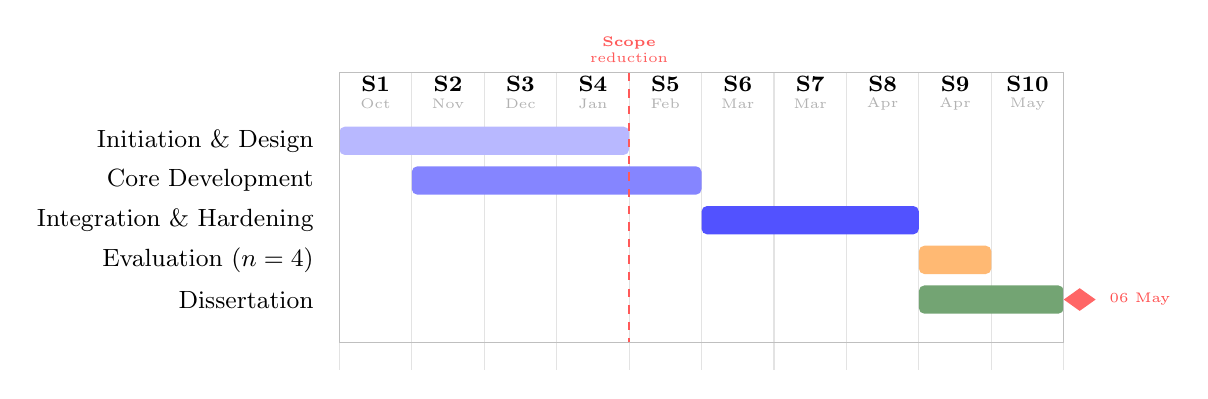
\begin{tikzpicture}[x=0.92cm, y=0.72cm]
  \foreach \x in {0,...,10} {
    \draw[gray!22, thin] (\x, 0.65) -- (\x, -4.60);
  }
  \foreach \i in {1,...,10} {
    \pgfmathsetmacro\xc{\i - 0.5}
    \node[font=\footnotesize\bfseries] at (\xc, 0.45) {S\i};
  }
  \foreach \xc/\mo in
      {0.5/Oct, 1.5/Nov, 2.5/Dec, 3.5/Jan, 4.5/Feb,
       5.5/Mar, 6.5/Mar, 7.5/Apr, 8.5/Apr, 9.5/May} {
    \node[font=\tiny, gray!60] at (\xc, 0.10) {\mo};
  }
  \fill[blue!28, rounded corners=2pt] (0,-0.30) rectangle (4,-0.80);
  \node[anchor=east, font=\small] at (-0.22,-0.55) {Initiation \& Design};
  \fill[blue!48, rounded corners=2pt] (1,-1.00) rectangle (5,-1.50);
  \node[anchor=east, font=\small] at (-0.22,-1.25) {Core Development};
  \fill[blue!68, rounded corners=2pt] (5,-1.70) rectangle (8,-2.20);
  \node[anchor=east, font=\small] at (-0.22,-1.95) {Integration \& Hardening};
  \fill[orange!55, rounded corners=2pt] (8,-2.40) rectangle (9,-2.90);
  \node[anchor=east, font=\small] at (-0.22,-2.65) {Evaluation ($n=4$)};
  \fill[green!35!black!55, rounded corners=2pt] (8,-3.10) rectangle (10,-3.60);
  \node[anchor=east, font=\small] at (-0.22,-3.35) {Dissertation};
  \draw[red!65, thick, dashed] (4, 0.65) -- (4,-4.10);
  \node[red!65, font=\tiny, align=center, above] at (4, 0.65)
      {\textbf{Scope}\\reduction};
  \fill[red!60]
      (10.00,-3.35) -- (10.22,-3.15) -- (10.44,-3.35) -- (10.22,-3.55) -- cycle;
  \node[anchor=west, font=\tiny, red!70] at (10.50,-3.35) {06~May};
  \draw[black!25] (0, 0.65) rectangle (10,-4.10);
\end{tikzpicture}
\caption{Project Gantt chart. Each column = one fortnightly sprint (Oct~2025--May~2026).
The red dashed line marks the Sprint~5 scope reduction.}
\label{fig:gantt}
\end{figure}

% ─────────────────────────────────────────────────────────────────────────────
\section{Risk Register}
\label{sec:meth_risks}
% ─────────────────────────────────────────────────────────────────────────────

\begin{table}[H]
\centering
\caption{Project risk register. L = Likelihood; I = Impact (H/M/L).}
\label{tab:risk_register}
\renewcommand{\arraystretch}{1.25}
\begin{tabularx}{\textwidth}{cp{4.0cm}ccp{2.0cm}X}
\toprule
\textbf{ID} & \textbf{Risk} & \textbf{L} & \textbf{I} & \textbf{Status} & \textbf{Mitigation} \\
\midrule
R1 & IRT 3PL fails to converge &
  H & M & Mitigated &
  Pre-specify Rasch fallback; fix $c=0.25$ \\
R2 & Participant attrition at follow-up &
  H & M & Accepted &
  Target $n=18$ recruitment; acknowledged in limitations \\
R3 & \texttt{variant\_pool\_\allowbreak exhausted} &
  M & L & Mitigated &
  Fallback to unrestricted pool; event emitted \\
R4 & Supabase RLS misconfiguration &
  L & H & Mitigated &
  RLS policies peer-reviewed; rate limiting on auth \\
R5 & BKT state corruption (concurrent sessions) &
  L & H & Mitigated &
  Postgres row-level locking; atomic session writes \\
R6 & Scope overrun (multi-domain) &
  H & H & Resolved &
  Sprint~5 scope reduction to single-domain Geography \\
\bottomrule
\end{tabularx}
\end{table}

% ─────────────────────────────────────────────────────────────────────────────
\section{What Was and Was Not Delivered}
\label{sec:meth_delivery}
% ─────────────────────────────────────────────────────────────────────────────

\subsection{Delivered}

\begin{itemize}[leftmargin=2em]
  \item Hybrid IRT 3PL + BKT adaptive engine with EAP estimation,
        Bloom-gated selection, and credit-factor BKT modification
  \item 13-KC question bank with isomorphic variants and cross-session deduplication
  \item Three-level graduated hint system with evidential credit weighting
  \item Pre-test seeding with Laplace-smoothed logit initialisation
  \item BKT decay detection and successive relearning boost ($1.5\times$)
  \item Five-tab session summary dashboard (Trajectory, Skills, Misconceptions, Achievements, Share)
  \item Leaderboard with XP ranking, consent opt-in, and rank-change animation
  \item First-visit onboarding tour
  \item Security implementation: bcrypt, JWT, rate limiting, Supabase RLS, NIST SP 800-63B compliance
  \item Production deployment on Vercel with Supabase Frankfurt backend
\end{itemize}

\subsection{Not Delivered}

\begin{itemize}[leftmargin=2em]
  \item \textbf{Multi-domain support.} Superseded by the Sprint~5 scope
        reduction; the architecture supports extension without algorithmic change.
  \item \textbf{K-means cold-start clustering.} Evaluated and superseded by
        pre-test seeding, which provides per-KC ability evidence rather than
        a demographic cluster assignment.
  \item \textbf{Full A/B randomised controlled trial.} VanLehn's meta-analytic
        benchmark used as comparator; static arm implemented but not wired.
  \item \textbf{7-day retention data at scale.} Follow-up data collection could
        not be completed within the project timeline.
\end{itemize}

% ─────────────────────────────────────────────────────────────────────────────
\section{Interface Design: Lo-fi Prototypes}
\label{sec:meth_lofi}
% ─────────────────────────────────────────────────────────────────────────────

Interface design preceded implementation in each sprint cycle.
Figure~\ref{fig:lofi_question} shows the lo-fi wireframe for the adaptive
question screen, and Figure~\ref{fig:lofi_summary} shows the session summary
dashboard layout. Both informed the production React component specifications
authored by the candidate.

\begin{figure}[H]
\centering
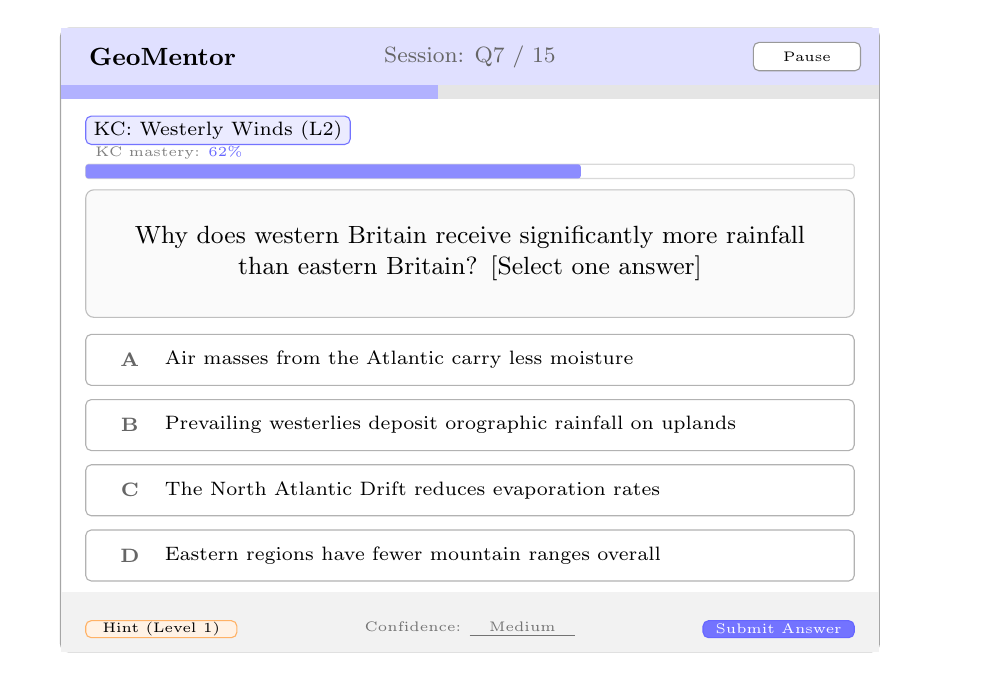
\begin{tikzpicture}[x=0.80cm, y=0.72cm]
  % Outer browser chrome
  \draw[black!35, rounded corners=3pt] (0,0) rectangle (13,-11);

  % Top navigation bar
  \fill[blue!12] (0,0) rectangle (13,-1.0);
  \node[anchor=west, font=\small\bfseries] at (0.3,-0.50) {GeoMentor};
  \node[font=\footnotesize, black!60] at (6.5,-0.50) {Session: Q7 / 15};
  \draw[black!40, rounded corners=2pt, fill=white] (11.0,-0.75) rectangle (12.7,-0.25);
  \node[font=\tiny] at (11.85,-0.50) {Pause};

  % Progress bar strip
  \fill[blue!30] (0,-1.0) rectangle (6.0,-1.25);
  \fill[gray!20] (6.0,-1.0) rectangle (13,-1.25);

  % KC badge + Bloom level
  \draw[blue!55, rounded corners=2pt, fill=blue!8]
    (0.4,-1.55) rectangle (4.6,-2.05);
  \node[font=\scriptsize] at (2.5,-1.80) {KC: Westerly Winds (L2)};

  % Mastery bar label
  \node[font=\tiny, black!50, anchor=west] at (0.4,-2.20)
    {KC mastery: {\color{blue!60}62\%}};
  \draw[gray!30, rounded corners=1pt] (0.4,-2.40) rectangle (12.6,-2.65);
  \fill[blue!45, rounded corners=1pt] (0.4,-2.40) rectangle (8.26,-2.65);

  % Question text box
  \draw[black!25, rounded corners=3pt, fill=gray!4]
    (0.4,-2.85) rectangle (12.6,-5.10);
  \node[font=\small, align=center, text width=11cm] at (6.5,-3.97)
    {Why does western Britain receive significantly more rainfall\\
     than eastern Britain? [Select one answer]};

  % Answer options
  \foreach \i/\lbl/\txt in {
    0/A/Air masses from the Atlantic carry less moisture,
    1/B/Prevailing westerlies deposit orographic rainfall on uplands,
    2/C/The North Atlantic Drift reduces evaporation rates,
    3/D/Eastern regions have fewer mountain ranges overall
  }{
    \pgfmathsetmacro\yy{-5.40 - \i*1.15}
    \draw[black!30, rounded corners=2pt, fill=white]
      (0.4,\yy) rectangle (12.6,\yy-0.90);
    \node[font=\scriptsize\bfseries, black!60] at (1.1,\yy-0.45) {\lbl};
    \node[font=\scriptsize, anchor=west, text width=10cm] at (1.5,\yy-0.45) {\txt};
  }

  % Bottom bar: Hint | Confidence | Submit
  \fill[gray!10] (0,-9.95) rectangle (13,-11);
  \draw[orange!60, rounded corners=2pt, fill=orange!10]
    (0.4,-10.45) rectangle (2.8,-10.75);
  \node[font=\tiny] at (1.6,-10.60) {Hint (Level 1)};
  \node[font=\tiny, black!55] at (6.5,-10.60)
    {Confidence: \underline{~~~Medium~~~}};
  \draw[blue!60, rounded corners=2pt, fill=blue!55]
    (10.2,-10.45) rectangle (12.6,-10.75);
  \node[font=\tiny, white] at (11.4,-10.60) {Submit Answer};
\end{tikzpicture}
\caption{Lo-fi wireframe: adaptive question screen. Key elements are the KC
  badge (identifies active Knowledge Component and Bloom level), the BKT
  mastery bar (reflects live $p(\text{Learned})$), four MCQ options, the
  graduated hint trigger (orange), confidence rating, and submit button.
  This wireframe preceded the Sprint~4 React implementation.}
\label{fig:lofi_question}
\end{figure}

\begin{figure}[H]
\centering
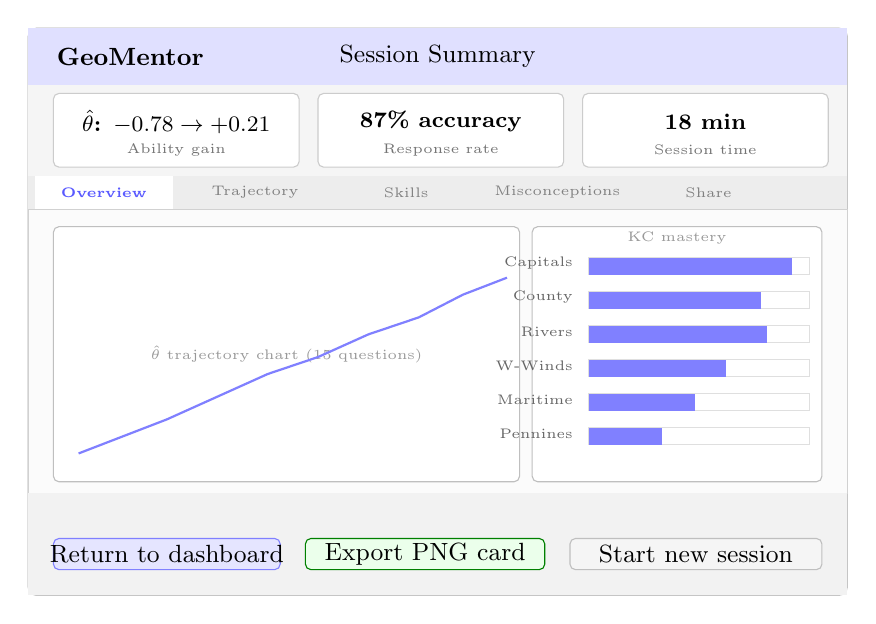
\begin{tikzpicture}[x=0.80cm, y=0.72cm]
  % Outer browser chrome
  \draw[black!35, rounded corners=3pt] (0,0) rectangle (13,-10);

  % Header bar
  \fill[blue!12] (0,0) rectangle (13,-1.0);
  \node[anchor=west, font=\small\bfseries] at (0.3,-0.50) {GeoMentor};
  \node[font=\small] at (6.5,-0.50) {Session Summary};

  % Stats strip: three stat boxes
  \fill[gray!8] (0,-1.0) rectangle (13,-2.6);
  \foreach \i/\statval/\statlbl in {
    0/{$\hat{\theta}$: $-0.78 \to +0.21$}/Ability gain,
    1/{87\% accuracy}/Response rate,
    2/{18 min}/Session time
  }{
    \pgfmathsetmacro\xleft{0.4 + \i*4.2}
    \pgfmathsetmacro\xright{\xleft + 3.9}
    \draw[black!20, rounded corners=2pt, fill=white]
      (\xleft,-1.15) rectangle (\xright,-2.45);
    \node[font=\footnotesize\bfseries] at (\xleft+1.95,-1.65) {\statval};
    \node[font=\tiny, black!55] at (\xleft+1.95,-2.15) {\statlbl};
  }

  % Tab bar
  \fill[gray!14] (0,-2.6) rectangle (13,-3.2);
  \foreach \i/\tabnm in {
    0/Overview, 1/Trajectory, 2/Skills, 3/Misconceptions, 4/Share
  }{
    \pgfmathsetmacro\tcx{1.2 + \i*2.4}
    \ifnum\i=0
      \fill[white] (\tcx-1.1,-2.6) rectangle (\tcx+1.1,-3.2);
      \node[font=\tiny\bfseries, blue!65] at (\tcx,-2.90) {\tabnm};
    \else
      \node[font=\tiny, black!50] at (\tcx,-2.90) {\tabnm};
    \fi
  }

  % Main content pane (Overview tab active)
  \draw[black!18, fill=gray!3] (0,-3.2) rectangle (13,-8.2);

  % Left: $\hat\theta$ trajectory chart placeholder
  \draw[black!25, fill=white, rounded corners=2pt]
    (0.4,-3.5) rectangle (7.8,-8.0);
  \node[font=\tiny, black!40] at (4.1,-5.75)
    {$\hat{\theta}$ trajectory chart (15 questions)};
  % Simulated line
  \draw[blue!50, thick]
    (0.8,-7.5) -- (1.5,-7.2) -- (2.2,-6.9) -- (3.0,-6.5)
    -- (3.8,-6.1) -- (4.6,-5.8) -- (5.4,-5.4) -- (6.2,-5.1)
    -- (6.9,-4.7) -- (7.6,-4.4);

  % Right: per-KC mastery bars
  \draw[black!25, fill=white, rounded corners=2pt]
    (8.0,-3.5) rectangle (12.6,-8.0);
  \node[font=\tiny, black!40, align=center] at (10.3,-3.70)
    {KC mastery};
  \foreach \j/\kcshort/\pct in {
    0/Capitals/0.92,
    1/County/0.78,
    2/Rivers/0.81,
    3/W-Winds/0.62,
    4/Maritime/0.48,
    5/Pennines/0.33
  }{
    \pgfmathsetmacro\ybase{-4.00 - \j*0.60}
    \node[anchor=east, font=\tiny, black!60] at (8.8,\ybase-0.15) {\kcshort};
    \draw[gray!25] (8.9,\ybase-0.05) rectangle (12.4,\ybase-0.35);
    \pgfmathsetmacro\barend{8.9 + \pct*3.5}
    \fill[blue!50] (8.9,\ybase-0.05) rectangle (\barend,\ybase-0.35);
  }

  % Bottom action bar
  \fill[gray!10] (0,-8.2) rectangle (13,-10);
  \draw[blue!50, rounded corners=2pt, fill=blue!10]
    (0.4,-9.0) rectangle (4.0,-9.55);
  \node[font=\small] at (2.2,-9.275) {Return to dashboard};
  \draw[green!50!black, rounded corners=2pt, fill=green!8]
    (4.4,-9.0) rectangle (8.2,-9.55);
  \node[font=\small] at (6.3,-9.275) {Export PNG card};
  \draw[gray!50, rounded corners=2pt, fill=gray!8]
    (8.6,-9.0) rectangle (12.6,-9.55);
  \node[font=\small] at (10.6,-9.275) {Start new session};
\end{tikzpicture}
\caption{Lo-fi wireframe: session summary dashboard (Overview tab active).
  The three-stat strip reports the within-session $\Delta\hat{\theta}$,
  overall accuracy, and session duration. Left pane: $\hat{\theta}$ trajectory
  chart across 15 questions. Right pane: per-KC BKT mastery bars.
  Tab navigation exposes Trajectory (interactive chart), Skills (KC breakdown),
  Misconceptions (distractor analysis), and Share (PNG card export).}
\label{fig:lofi_summary}
\end{figure}

% ─────────────────────────────────────────────────────────────────────────────
\section{Quality Assurance}
\label{sec:meth_qa}
% ─────────────────────────────────────────────────────────────────────────────

Quality assurance mechanisms employed include: TypeScript strict mode
eliminating runtime errors at the type-checking stage; Prisma migration files
providing a versioned schema audit trail; Vercel preview deployments enabling
integration testing per feature branch before merge; and Supabase RLS
verification by cross-user access testing from a test account.
